\label{sec:radicals}
\section{Radicals}
$$ \sqrt[n]{x} $$
\begin{itemize}
  \item $x$ is the \textbf{radicand}.
  \item $n$ is the \textbf{index}(nth root).
  \item $ \sqrt[n]{x}$ expression is the \textbf{radical}
\end{itemize}

As promised let's look at the fractional exponent equation. If $n$ is a positive integer that is greater than $1$ and a is a real number then,
$$ \sqrt[n]{a} = a^{\frac{1}{n}} $$

We are often referring the left side of the equation as the \textbf{radical form} and the right side of the equation as the \textbf{exponent form}

\subsubsection{Proof}
In order to prove this equation we can establish first this: 
$$ (a^{\frac{1}{n}})^{n} = a^{n \cdot \frac{1}{n}} = a^{\frac{n}{n}} = a $$
Let's take an example to avoid confusion: 
$$ (9^{\frac{1}{2}})^2 = 9^{\frac{1}{2} \cdot2} = 9^{\frac{2}{2}} = 9 $$

To put this into words $ 9^{\frac{1}{2}} $ is the number that when squared will return back $ 9 $. In other words this is exactly what it meant by the root(in this case square root) which will return back the number that when squared it will be 9. Therefore: 
$$ 9^{\frac{1}{2}} =  \sqrt[2]{9} = 3 $$

Since,
$$ (3)^2 = 9 = (9^{\frac{1}{2}})^2 $$

Therefore the equation has been proven: 
$$ \sqrt[n]{a} = a^{\frac{1}{n}} $$

It is very important to note a misconception here. The index is required in these radical expressions to make sure that we correctly evaluate the radical. There is one exception to this rule and that is square root.
$$ \sqrt[2]{a} = \sqrt[]{a} $$
In every other cases we \textbf{must} define the index, because otherwise it will be considered as a square root, Whenever working with square roots the index can be omitted.

\subsubsection{General rational exponent}
Since, $ a^{\frac{1}{n}} = \sqrt[n]{a} $.
Let's establish the general rational exponent in terms of radicals as follows. 
$$ a^{\frac{m}{n}} = (a^{\frac{1}{n}}) ^{m} = (\sqrt[n]{a})^m $$
$$ OR $$
$$ a^{\frac{m}{n}} = (a^m) ^{\frac{1}{n}} = \sqrt[n]{a^m} $$

Since being aware of the \textbf{Associative Property of Multiplication}, the order of the multiplication can be changed. 

Therefore, 
$$ a^{\frac{m}{n}} = \sqrt[n]{a^m} $$

\subsection{Properties of radicals}
\begin{itemize}
  \item $\sqrt[n]{a^n} = a$ \ This is simply true because when trying to find the $n$th root of a number and  also raising the number to that power then that's simply will be equal to the number.  \\
Consider this as an example,
$$ \sqrt[]{9^2} = \sqrt[]{81} = 9$$
   \item $ \sqrt[n]{ab} = \sqrt[n]{a} \sqrt[n]{b} $ \\
   To prove this consider this, \\
    1. Start with the left-hand side (LHS) of the equation,
    $ \sqrt[n]{ab} $ Using the definition of the nth root:
    $ \sqrt[n]{ab} = (ab)^{\frac{1}{n}} $ \\
    2. Next apply the product rule of exponents, which states that $ a^m \cdot a^n = a^{m+n} $ Therefore, $ (ab)^{\frac{1}{n}} = a^{\frac{1}{n}} \cdot b^{\frac{1}{n}} $ \\ 
    3. Now, rewrite the exponents as radicals:
    $ a^{\frac{1}{n}} $ is equivalent to $ \sqrt[n]{a} $ and $ b^{\frac{1}{n}} $ is equivalent to $ \sqrt[n]{b} $ \\
    4. So, we have: $ a^{\frac{1}{n}} \cdot b^{\frac{1}{n}} = \sqrt[n]{a} \cdot \sqrt[n]{b} $ \\
    5. Finally this proves that: $ \sqrt[n]{ab} = \sqrt[n]{a} \cdot \sqrt[n]{b} $
    \item $ \sqrt[n]{\frac{a}{b}} = \frac{\sqrt[n]{a}}{\sqrt[n]{b}} $ To prove this consider this, \\
    1. As previously Start with the left-hand side (LHS) of the equation: $ \sqrt[n]{\frac{a}{b}} $ \\
    2. Now using the definition of the nth root: $ \sqrt[n]{\frac{a}{b}} = \left(\frac{a}{b}\right)^{\frac{1}{n}} $ \\
    3. Apply the power rule of the exponents which states that: \\ $ (a^m)^{\frac{1}{n}} = a^{m \cdot \frac{1}{n}} = a^{\frac{m}{n}}$, Therefore when we are dealing with a fraction as the base it is the same when dealing with numbers that are not fractions: 
$$ \left(\frac{a}{b}\right)^{\frac{1}{n}} = \frac{a^{\frac{1}{n}}}{b^{\frac{1}{n}}} $$ Since, \\
$$ (\frac{a}{b})^c = \frac{a^c}{b^c} $$ \\
With an example: $ (\frac{a}{b})^2 = \frac{a}{b} \cdot \frac{a}{b} = \frac{a^2}{b^2} $ \\
	4. Now rewrite the exponents as radicals: $ a^{\frac{1}{n}} $ is equivalent to $ \sqrt[n]{a} $ and  $b^{\frac{1}{n}}$ is equivalent to $ \sqrt[n]{b} $ \\
	5. So, we have: 
	$$ \frac{a^{\frac{1}{n}}}{b^{\frac{1}{n}}} = \frac{\sqrt[n]{a}}{\sqrt[n]{b}} $$ \\
	6. Finally, this proves that: 
	$$ \sqrt[n]{\frac{a}{b}} = \frac{\sqrt[n]{a}}{\sqrt[n]{b}} $$ \\
	\\
	
	\item Also note that while we can “break up” products and quotients under a radical we can’t do the same thing for sums or differences. In other words,
	$$ \sqrt[n]{a+b} \neq \sqrt[n]{a}+ \sqrt[n]{b}  $$ 
	$$ AND $$
	$$ \sqrt[n]{a-b} \neq \sqrt[n]{a}- \sqrt[n]{b} $$ \\
These can simply be proven by examples, 
$$ 5 = \sqrt25 = \sqrt{9+16} \neq \sqrt9 + \sqrt16 = 3+4 = 7 $$

\begin{align*}
  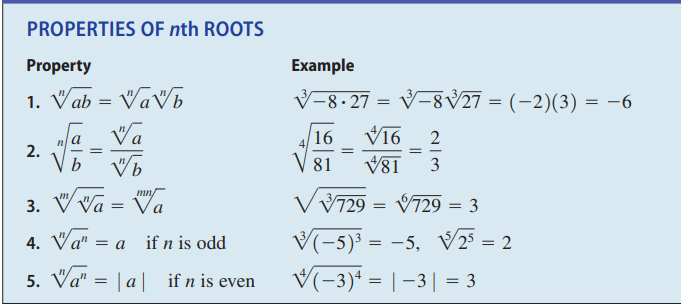
\includegraphics[width=0.8\textwidth]{algebra-pre-calculus/algebra/radicals/properties_of_nth_roots.png}
\end{align*}

\end{itemize}
\subsection{Using the Laws of Exponents with Rational Exponents}
(a) \scalebox{1.1}{$a^{1 / 3} a^{7 / 3}=a^{8 / 3}$} $\Rightarrow$
\textbf{Law 1: $a^m a^n=a^{m+n}$} \\ \break
(b) \scalebox{1.1}{$\frac{\displaystyle a^{2 / 5} a^{7 / 5}}{a^{3 / 5}}=a^{2 / 5+7 / 5-3 / 5}=a^{6 / 5}$} $\Rightarrow$
\textbf{Law 1, Law 2:} $\frac{a^m}{a^n}=a^{m-n}$ \\ \break
(c)
$$
\begin{aligned}
\left(2 a^3 b^4\right)^{3 / 2} & =2^{3 / 2}\left(a^3\right)^{3 / 2}\left(b^4\right)^{3 / 2} \\
& =(\sqrt{2})^3 a^{3(3 / 2)} b^{4(3 / 2)} \\
& = \sqrt{2^2} \cdot \sqrt{2} \cdot a^{9 / 2} b^{6} \\
& =2 \sqrt{2} \cdot a^{9 / 2} \cdot b^6
\end{aligned}
$$
\textbf{Law 4:} $(a b c)^n=a^n b^n c^n$ \\
\textbf{Law 3:} $\left(a^m\right)^n=a^{m n}$ \\ \break
(d)
$$
\begin{aligned}
\left(\frac{2 x^{3 / 4}}{y^{1 / 3}}\right)^3 \cdot \left(\frac{y^4}{x^{-1 / 2}}\right) & =\frac{2^3\left(x^{3 / 4}\right)^3}{\left(y^{1 / 3}\right)^3} \cdot\left(y^4 x^{1 / 2}\right) \\
& =\frac{8 x^{9 / 4}}{y} \cdot y^4 x^{1 / 2} \\
& =8 x^{11 / 4} y^3
\end{aligned}
$$
\textbf{Laws 5, 4, and 7 \\
Law 3 \\
Laws 1 and 2}

\subsection{Simplifying by Writing Radicals as Rational Exponents}
\textbf{(a)} $\displaystyle \frac{1}{\sqrt[3]{x^4}}=\frac{1}{x^{4 / 3}}=x^{-4 / 3} \Rightarrow$ Definition of rational and negative exponents \\ \break
\textbf{(b)} $(2 \sqrt{x})(3 \sqrt[3]{x})=\left(2 x^{1 / 2}\right)\left(3 x^{1 / 3}\right)$ $=6 x^{1 / 2+1 / 3}=6 x^{5 / 6} \Rightarrow$ Definition of rational exponents \\ \break 
\textbf{(c)}
$$
\begin{aligned}
\sqrt{x \sqrt{x}} & =\left(x x^{1 / 2}\right)^{1 / 2} \\
& =\left(x^{3 / 2}\right)^{1 / 2} \\
& =x^{3 / 4}
\end{aligned}
$$

\textbf{Law 1}
\textbf{Definition of rational exponents} \\
\textbf{Law 1} \\
\textbf{Law 3} \\

\subsection{Rationalizing the Denominator; Standard Form}
It is often useful to eliminate the radical in a denominator by multiplying both numerator and denominator by an appropriate expression. This procedure is called \textbf{rationalizing the denominator}. If the denominator is of the form $\sqrt{a}$, we multiply numerator
and denominator by $\sqrt{a}$. In doing this we multiply the given quantity by 1, so we do
not change its value. For instance,

$$
\displaystyle \frac{1}{\sqrt{a}}=\frac{1}{\sqrt{a}} \cdot 1=\frac{1}{\sqrt{a}} \cdot \frac{\sqrt{a}}{\sqrt{a}}=\frac{\sqrt{a}}{a}
$$
Note that the denominator in the last fraction contains no radical. In general, if the denominator is of the form $\sqrt[n]{a^m}$ with $m<n$, then multiplying the numerator and denominator by $\sqrt[n]{a^{n-m}}$ will rationalize the denominator, because (for $a>0$ )

\begin{align*}
  \scalebox{1.3}{$
\displaystyle \sqrt[n]{a^m} \sqrt[n]{a^{n-m}}=\sqrt[n]{a^{m+n-m}}=\sqrt[n]{a^n}=a
$}
\end{align*}

The idea behind this is that when you subtract $n-m$ what you are doing is looking for the number that when you add with $m$ you are going to get $n$ and by doing so, whenever you have $\sqrt[n]{a^m} \sqrt[n]{a^{n-m}}$ this part since you have the same base you can just add the exponents up like this: $ \sqrt[n]{a^{m+n-m}} $ and since $ m+n-m = n $ then you will have $ \sqrt[n]{a^n} $ and since the $ n $th root and the $ n $th power cancel each other out you will be left with $ a $.

With an example, let's say that we have $a=4$ and $n=3$ and $m=1$ then we have:
$$ \sqrt[3]{4^1} \sqrt[3]{4^{3-1}} = \sqrt[3]{4^1} \sqrt[3]{4^2} = \sqrt[3]{4^3} = 4 $$
When we have subtracted $ 3-1 $ we have found the number that when we add with $ 1 $ we will get $ 3 $ and that number is $ 2 $ and since we have the same base we can just add the exponents up and we will get $ 3 $ and since the $ 3 $rd root and the $ 3 $rd power cancel each other out we will be left with $ 4 $. 
In conclusion we are always trying to find the number that when we add with $ m $ we will get $ n $ and that number is $ n-m $ and since we have the same base we can just add the exponents up and we will get $ n $ and since the $ n $th root and the $ n $th power cancel each other out we will be left with $ a $. 

\subsubsection{Examples of Rationalizing the Denominator}
Put each fractional expression into Standard form by rationalizing the denominator. \\
\textbf{(a)} $\displaystyle \frac{2}{\sqrt{3}}=\frac{2}{\sqrt{3}} \cdot \frac{\sqrt{3}}{\sqrt{3}}=\frac{2\sqrt{3}}{\sqrt{3\cdot3}}=\frac{2\sqrt{3}}{\sqrt{9}}=\frac{2\sqrt{3}}{3}$ \\ 
Here we have multiplied numerator and denominator by $\sqrt{3}$, which is the denominator of the given fraction. By doing so we got rid of the radical in the denominator. \\
\textbf{(b)} $\displaystyle \frac{1}{\sqrt[3]{5}}=\frac{1}{\sqrt[3]{5}} \cdot \frac{\sqrt[3]{5^2}}{\sqrt[3]{5^2}}=\frac{\sqrt[3]{5^2}}{\sqrt[3]{5\cdot5^2}}=\frac{\sqrt[3]{5^2}}{\sqrt[3]{5^3}}=\frac{\sqrt[3]{25}}{5}$ \\
Here we have multiplied numerator and denominator by $\sqrt[3]{5^2}$, the reason why is because when we are dealing with a cube root we are looking for the number that when we add with $ 1 $(which comes from the $5$'s exponent  $\sqrt[3]{5}$) we will get $ 3 $ and that number is $ 2 $ so that's why $\sqrt[3]{5^2}$, and since we have the same base we can just add the exponents up and we will get $ 3 $. and since the $ 3 $rd root and the $ 3 $rd power cancel each other out we will be left with $ 5 $. \\
\textbf{(c)} $\displaystyle \sqrt[7]{\frac{1}{a^2}} = \frac{1}{\sqrt[7]{a^2}} = \frac{1}{\sqrt[7]{a^2}} \cdot \frac{\sqrt[7]{a^5}}{\sqrt[7]{a^5}} = \frac{\sqrt[7]{a^5}}{\sqrt[7]{a^7}} = \frac{\sqrt[7]{a^5}}{a}$ \\
Here we have multiplied numerator and denominator by $\sqrt[7]{a^5}$, the reason why is because when we are dealing with a $ 7 $th root we are looking for the number that when we add with $ 2 $(which comes from the $a$'s exponent in $a^2$) we will get $ 7 $ and that number is $ 5 $ so that's why $\sqrt[7]{a^5}$, and since we have the same base we can just add the exponents up and we will get $ 7 $. and since the $ 7 $th root and the $ 7 $th power cancel each other out we will be left with $ a $. \\